\section{Gestione analisi}
	Per quanto riguarda la gestione delle \mglo{Analisi}{analisi}, l'utente ha la possibilità di:
	\begin{itemize}
		\item avviare un'analisi su certi scenari e visualizzare i risultati dell'analisi (sia in forma testuale sia su mappa) relativi agli scenari precedentemente scelti;
		\item cambiare l'anno di riferimento dei risultati di analisi (dopo 1, 2, o 3 anni) visualizzando i risultati dell'analisi aggiornati;
		\item cancellare risultati di analisi relativi a certi scenari su cui è stata calcolata una analisi.
	\end{itemize}
	
		\begin{figure}[H]
			\centering
			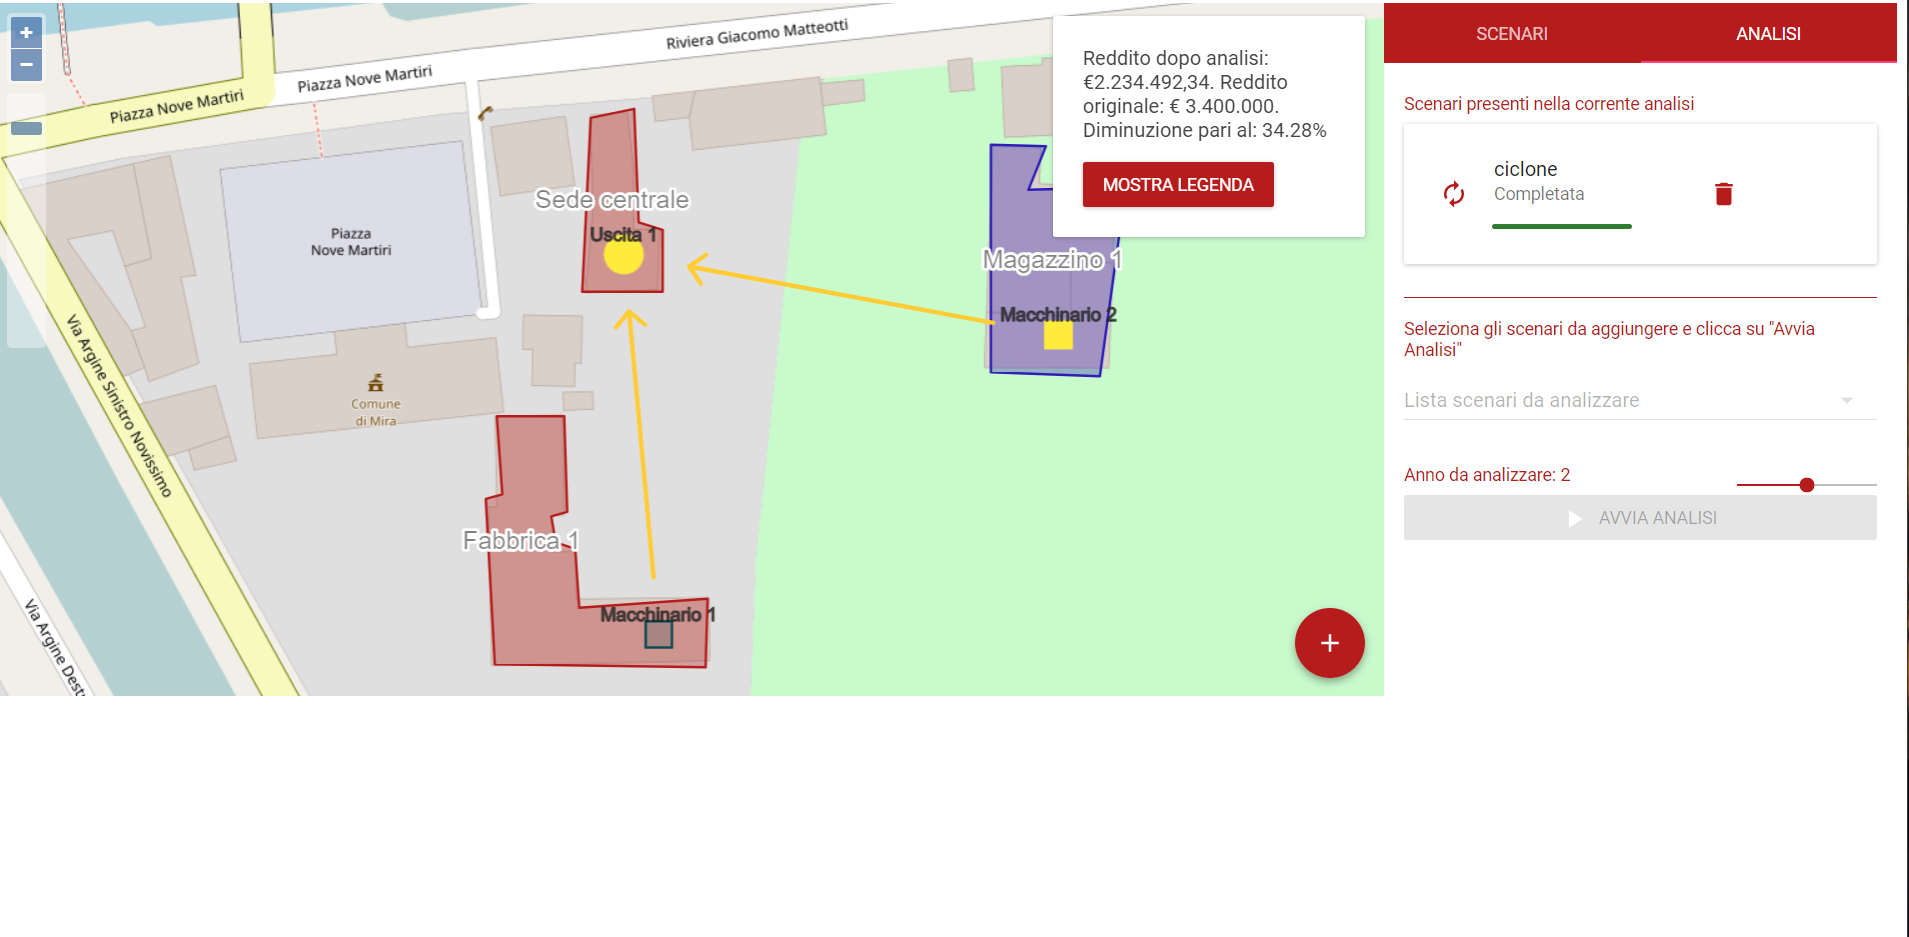
\includegraphics[width=\textwidth]{img/analisi.png}
			\caption{Menu di aggiunta}
		\end{figure}
		
\subsection{Avvio dell'analisi}
	Per avviare un'analisi di danno si deve:
	\begin{itemize}
		\item cliccare sulla lista di scenari da analizzare nella sidebar;
		\item selezionare uno o più scenari dal menù a tendina che si sarà aperto;
		\item premere sul pulsante "Avvia analisi".
	\end{itemize}

	\begin{figure}[H]
		\centering
		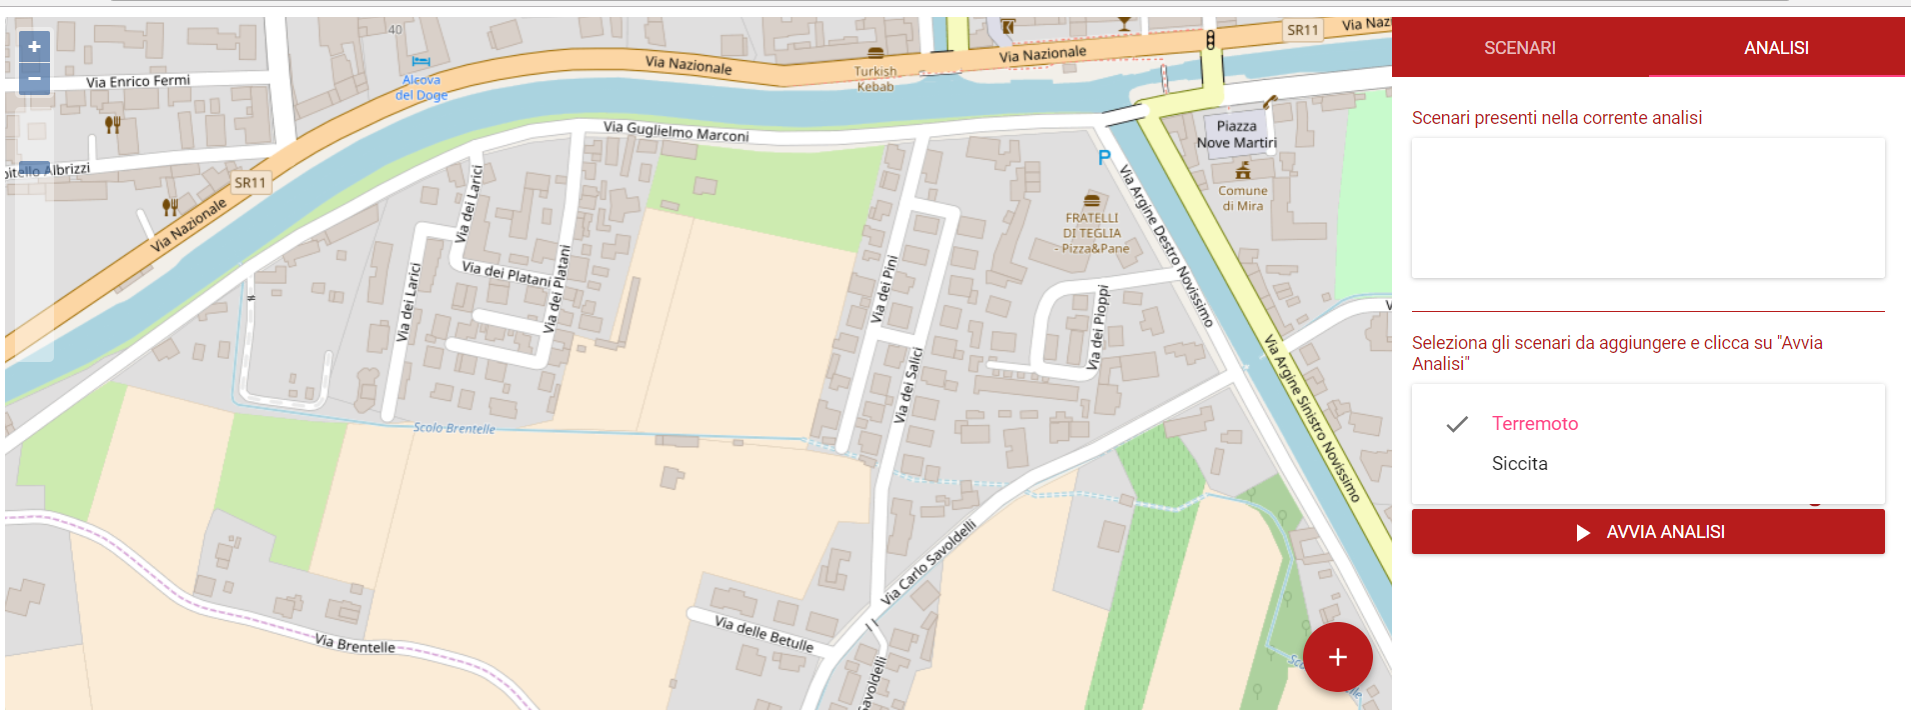
\includegraphics[width=\textwidth]{img/avvio_analisi.png}
		\caption{Avvio dell'analisi}
	\end{figure}

\subsection{Avanzamento analisi}
	Una volta avviata un'analisi, i suoi risultati non sono immediatamente disponibili, dato che è necessario del tempo per portare a termine il calcolo. L'avanzamento di questa operazione è visualizzato dalla barra presente nella sidebar.
	
	\begin{figure}[H]
		\centering
		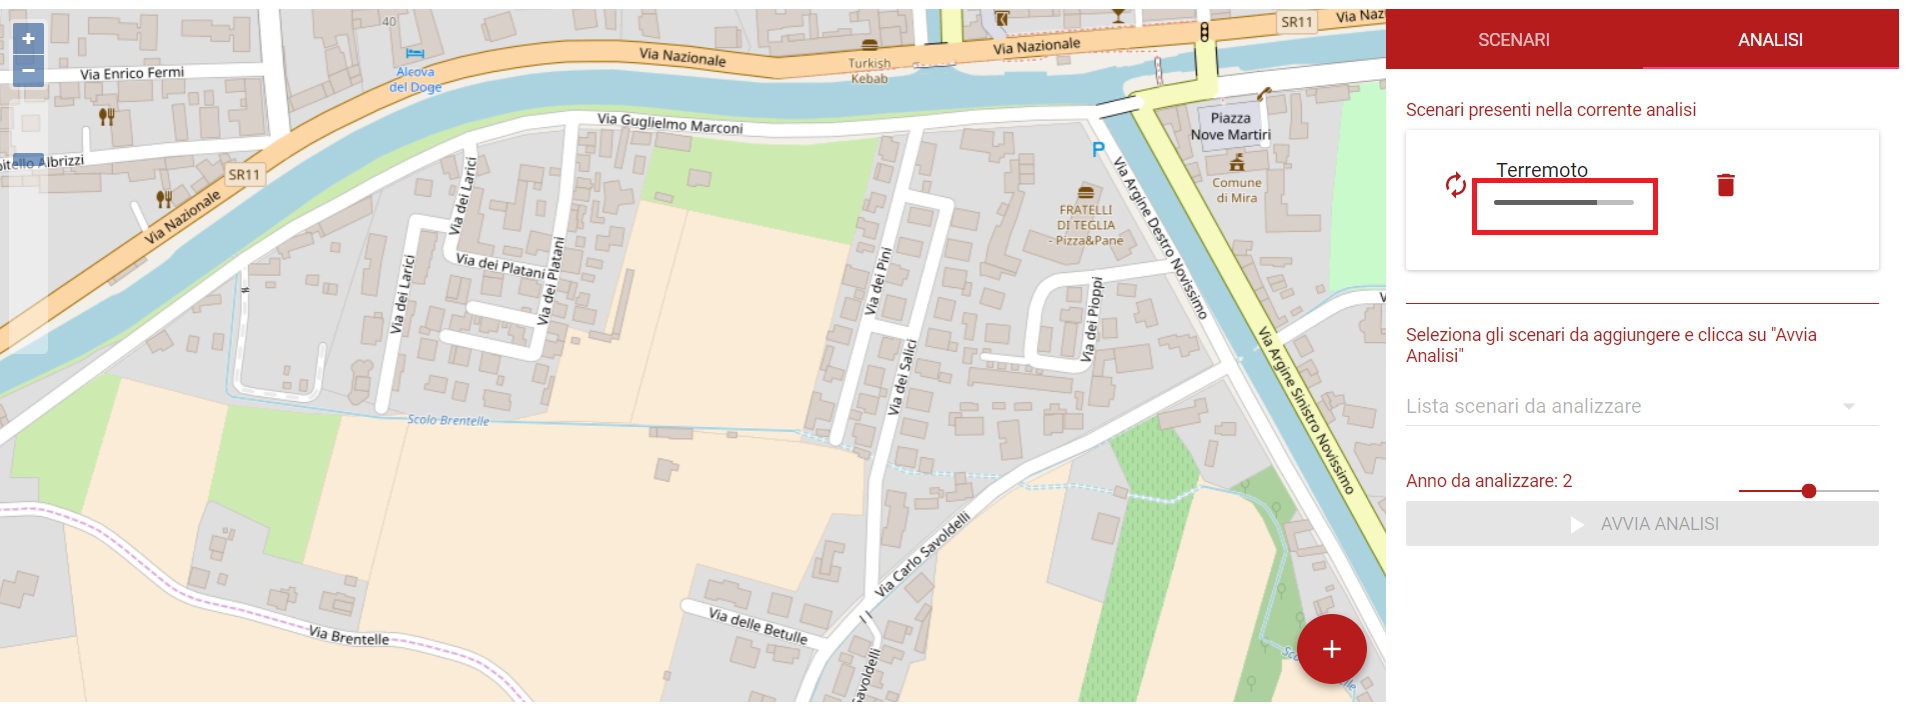
\includegraphics[width=\textwidth]{img/avanzamento_analisi.png}
		\caption{Avanzamento analisi}
	\end{figure}

\subsection{Risultati analisi e legenda}
	Quando l'analisi è completa, viene visualizzata una finestra informativa con i risultati economici dei danni causati dagli scenari presi in esame.
	Inoltre, sulla mappa i nodi assumono vari colori, a seconda della perdita economica che il nodo subisce.\\
	Cliccando sul pulsante "Mostra legenda" è possibile visualizzare una legenda che descrive il significato dei colori.

	\begin{figure}[H]
		\centering
		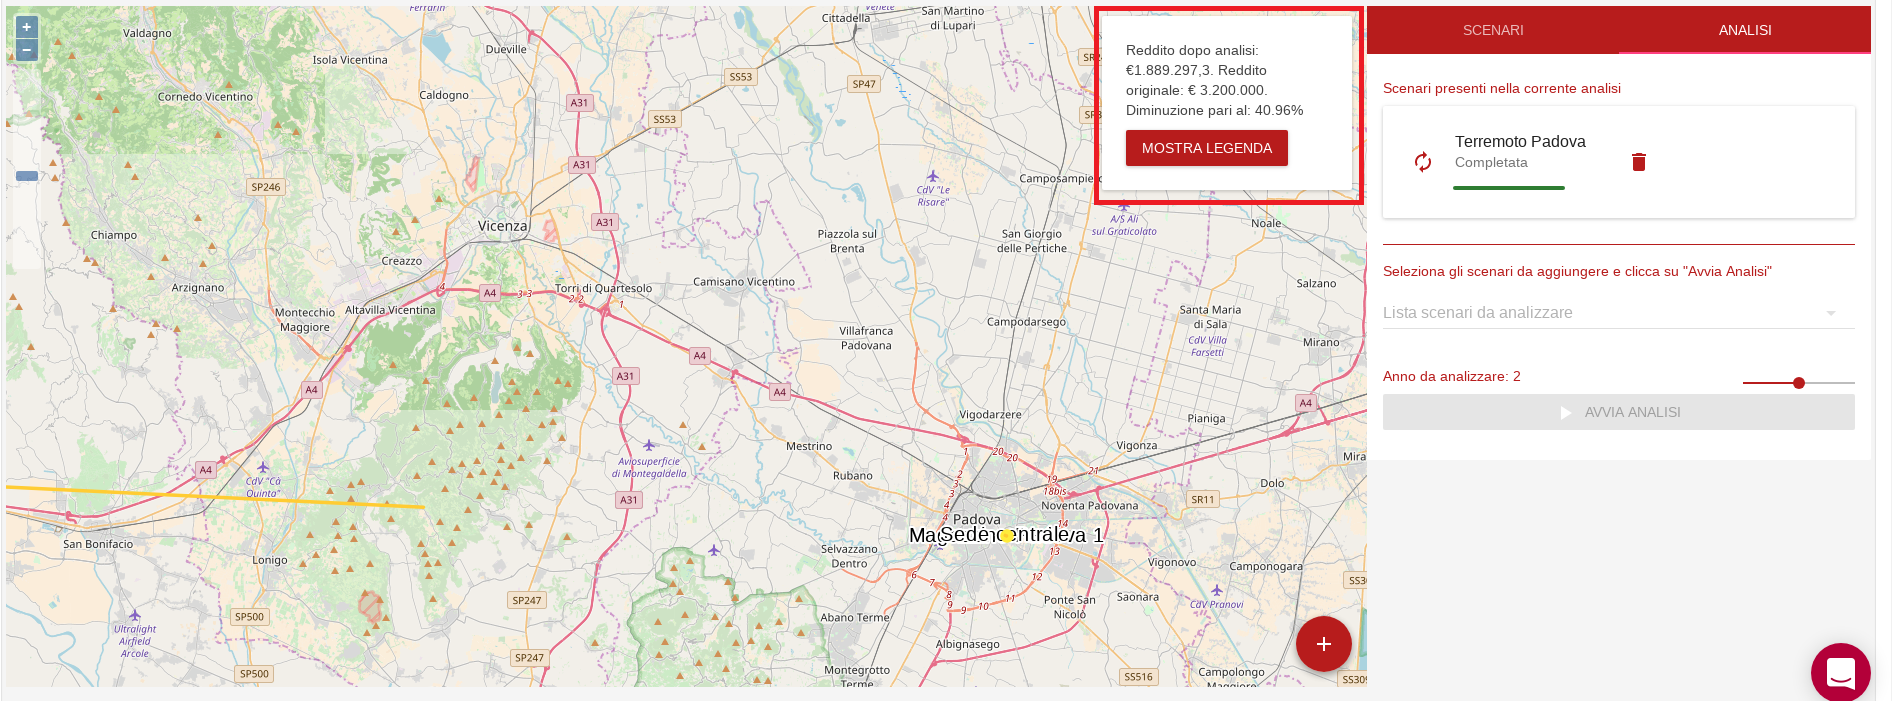
\includegraphics[width=\textwidth]{img/finestra_economica.png}
		\caption{Finestra risultati economici}
	\end{figure}

	\begin{figure}[H]
	\centering
	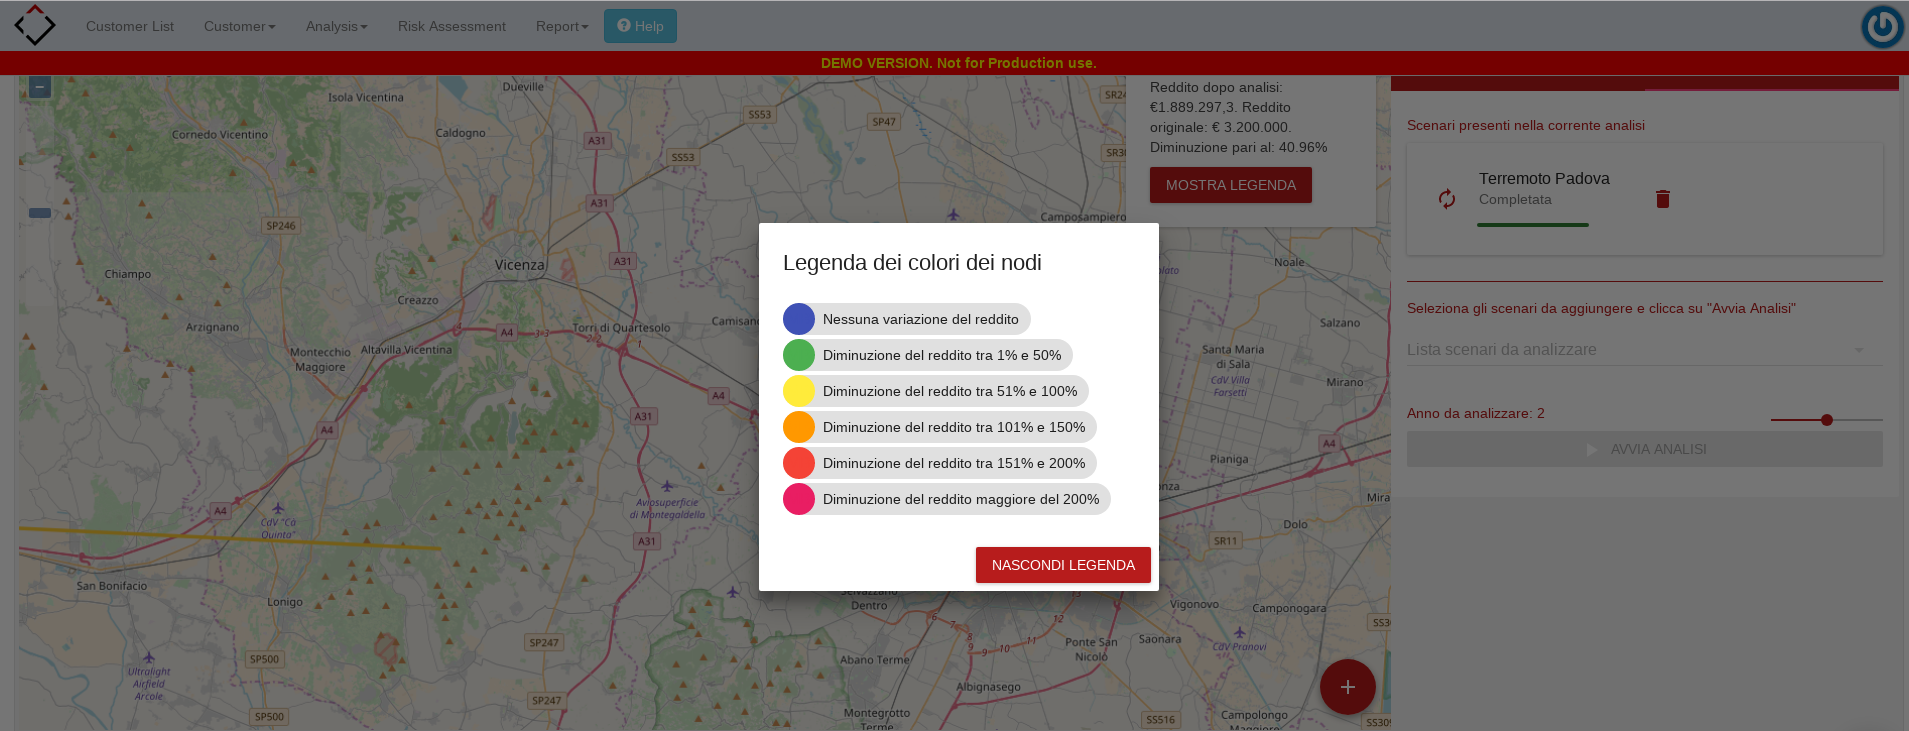
\includegraphics[width=\textwidth]{img/legenda_colori.png}
	\caption{Legenda colori nodi}
	\end{figure}

\subsection{Modifica anno di analisi}
	L'applicazione permette di visualizzare i risultati di danno a uno, due o tre anni a partire dalla data attuale. Per modificare l'anno di analisi, è possibile fare scorrere lo slider presente nella sidebar.
	
	\begin{figure}[H]
		\centering
		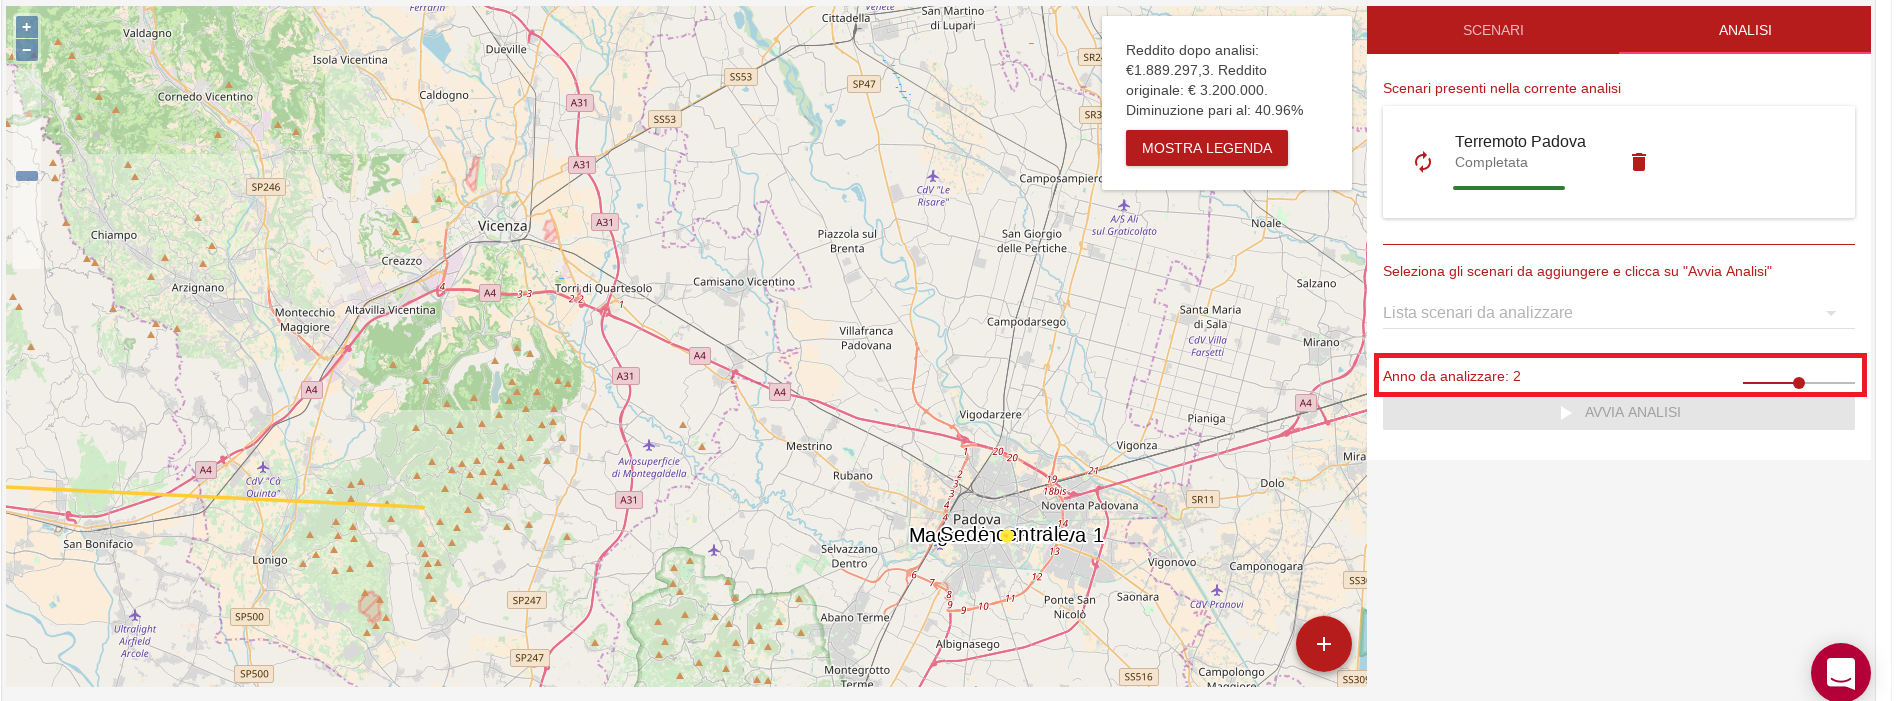
\includegraphics[width=\textwidth]{img/modifica_anno_analisi.png}
		\caption{Modifica anno di analisi}
	\end{figure}

\subsection{Cancellazione risultati di analisi}
	Per cancellare un'analisi, è possibile cliccare sul pulsante a forma di cestino sulla destra di ogni analisi.
	
	\begin{figure}[H]
		\centering
		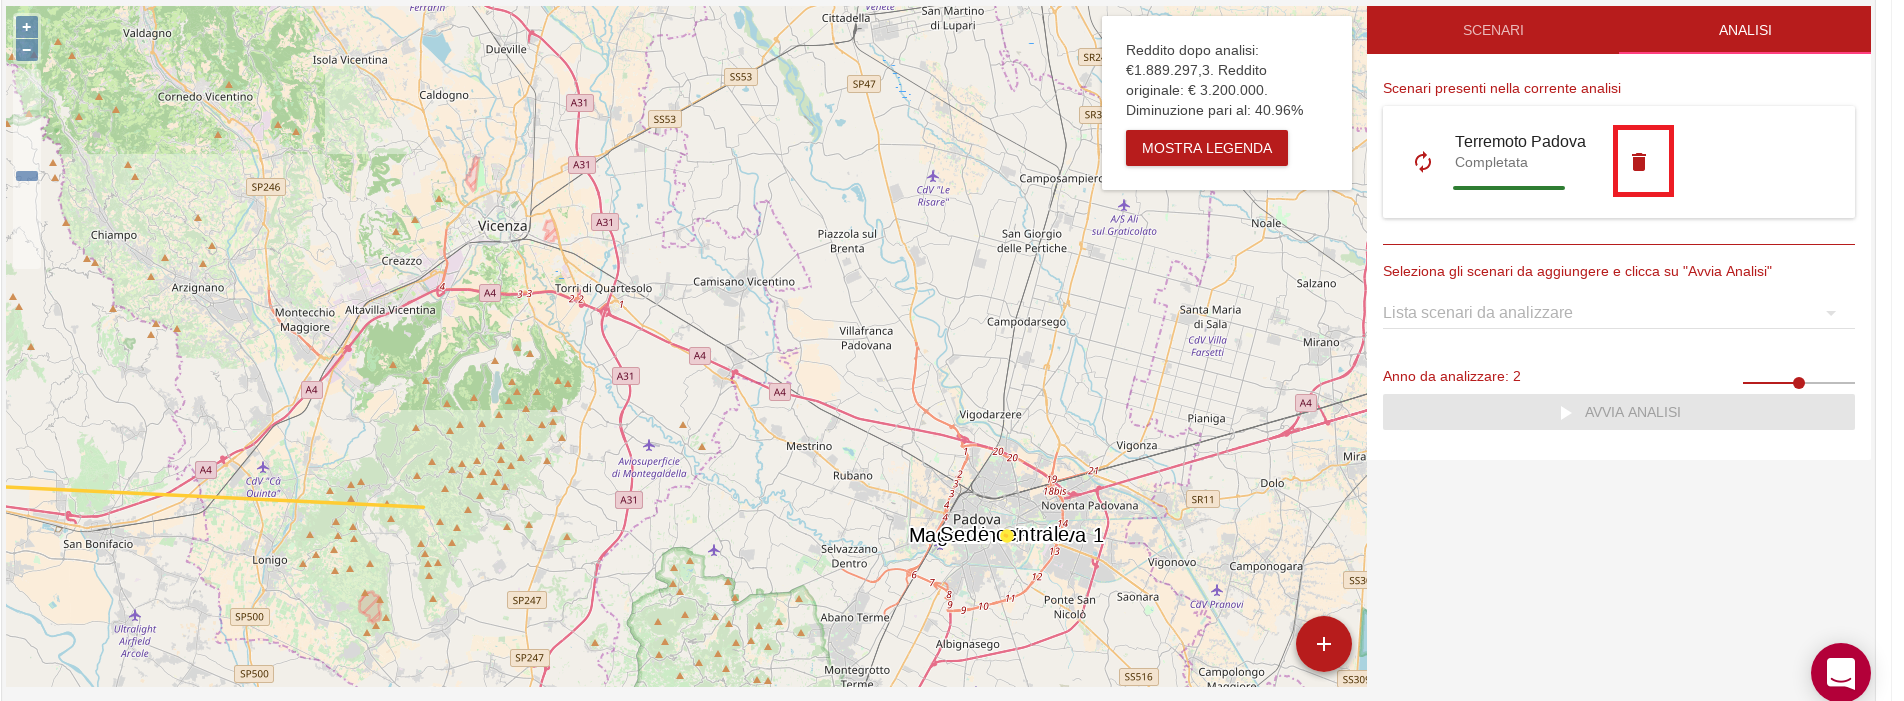
\includegraphics[width=\textwidth]{img/cancellazione_analisi.png}
		\caption{Cancellazione analisi}
	\end{figure}


\subsection{Riesecuzione analisi}
	Qualora i dati del processo produttivo o dello scenario fossero cambiati, è possibile ricalcolare l'analisi premendo sul pulsante con le due frecce a sinistra di ogni analisi.
	
	\begin{figure}[H]
		\centering
		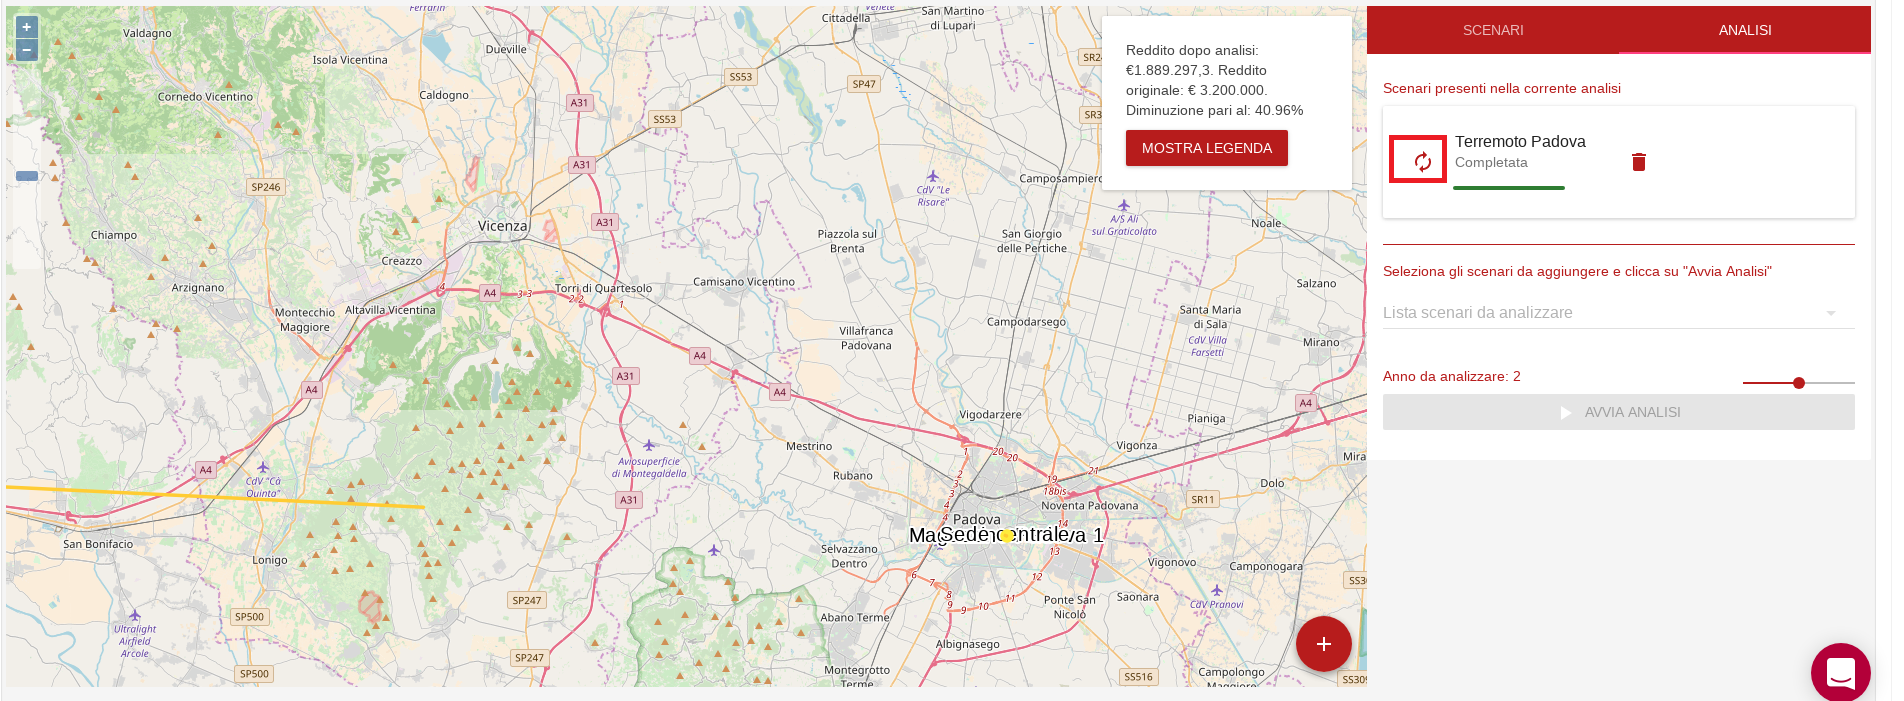
\includegraphics[width=\textwidth]{img/riesecuzione_analisi.png}
		\caption{Riesecuzione analisi}
	\end{figure}

